% template!!
\documentclass[sigconf,anonymous]{acmart}

\usepackage{booktabs}
\usepackage{amsmath}
\usepackage[linesnumbered,boxed]{algorithm2e}
\usepackage{subfigure}
\usepackage{epstopdf}
\usepackage{graphicx}
\usepackage{color}
\usepackage{multirow}
\usepackage{colortbl}
%\usepackage{ntheorem}
%\theoremseparator{:}
\theoremstyle{definition}
\newtheorem{hyp}{Hypothesis}
\newtheorem{mydef}{Definition}

\setcopyright{rightsretained}

\begin{document}

\title{How to Find Goals? Insight into the Wisdom of User Based on E-commerce Search Sessions}

\begin{abstract}
...


\end{abstract}


\keywords{...}

\maketitle
\section{Introduction}\label{sec:introduction}
...


\section{Related Work}\label{sec:related}
...

\section{Definitions and Data}\label{sec:definition}
In this section, we first introduce the definition of the \emph{search sessions}, \emph{search strategies} and \emph{search tags} in e-commerce. We then describe how to construct session data from a e-commerce search log and give statistics for the data set. Finally, we present the distribution of data set and compare them to traditional web search.

\subsection{Search Sessions}\label{sec:definition:session}
In the field of e-commerce, the system typically creates, stores and terminates a new active session with simple triggering rules. This is, the user opens the page (or application) as a signal to create, and closing the web page (or application) indicates termination. All actions during this time period would be stored, including the search logs we are interested in. The actions involved in the search include entering query keywords, clicking on items, and operating on the items, i.e. add to favourite, add to cart and purchase. However, this means that a user continuously searches for different goals when he does not close the page, such as T-shirts and jeans, and only one actual session is counted. Direct analysis on raw data can lead to ambiguous results. 

Since we are interested in the strategy that users take in the process of finding a goal, we need a different definition of the session to ensure the continuity of the search behavior and the consistency of the search target. This is similar to the problem of detecting session boundaries~\cite{Silverstein1999Analysis,He2002Combining,Jansen2006How,Jones2008Beyond,Lucchese2011Identifying,Liao2012Evaluating}. Most existing work identifies session boundaries using time constraints, where the interval between two adjacent actions cannot exceed a preset threshold $\theta_t$~\cite{Silverstein1999Analysis,He2002Combining,Jansen2006How}. This method is simple and intuitive, because if the user's next action is too far from the previous one, his intentions are likely to have changed. But this method suffers from the question of determining reasonable parameters. As the previous work presented, when the threshold was set to 5, 10 and 30 minutes, the best results were obtained for different experimental data~\cite{Silverstein1999Analysis,He2002Combining,Jansen2006How}. An unreasonable threshold would also result in a split session containing multiple goals.

Considering the above shortcomings, ~\cite{Jones2008Beyond,Lucchese2011Identifying,Liao2012Evaluating} proposes to use \emph{tasks} to characterize a user's goal and further extract a task-based session. This method guarantees the consistency of the session to a certain extent, but requires a lot of extra calculations. For instance, ~\cite{Jones2008Beyond} needs to construct a classifier based on features such as keywords and search results, and ~\cite{Lucchese2011Identifying} needs to combine text and semantic features to calculate similarity. Fortunately, in an e-commerce scenario, the item clicked by the user provides a new perspective to discover the user's goal. Assuming that a user continues to search and click on different T-shirts, we naturally think that his goal is to buy a T-shirt. On the other hand, using the clicked item to determine the consistency of the goal does not lead to additional calculations.

Based on above discussion, it is sound to define session by constrain both time and goal. We define \emph{search sessions} in the following way:
\begin{mydef}\label{def:session}
A \emph{Search Session} is a sequence of actions that are generated by a user for a specific goal over a continuous period of time.
\end{mydef}

Let $S$, $q$, $c$, $o$ and $G$ represent the search session, query keywords, clicked items, operations on the items and a specific goal respectively, the definition can be formalized as $S_i=\{(q_1,<c_1,o_1>), (q_2,<c_2,o_2>), ..., (q_n,<c_n,o_n>)\}$, where $|t_{q_j}-t_{q_i}|<\theta_t$ and $\{c_1,c_2,...,c_n\}\in G$. It should be noted that $c_i$ would contain one or more items, and $o_i$ would be a null value when the corresponding item is not operated. 

\subsection{Search Strategies and Search Tags}\label{sec:definition:tag}
Based on Def.~\ref{def:session}, a search session consists of search keywords, clicks and additional operations. Since the operation implicitly reflects the user's satisfaction with the item and is unknown to the user in advance, the variables that the user directly manipulates in the search session are the remaining two. We define the \emph{search strategies} as follows:
\begin{mydef}\label{def:strategy}
A \emph{Search Strategy} refers to how users coordinate search keywords and click behavior to better hit the goal.
\end{mydef}
There are two sources of strategy: the experience gained from the long-term interaction between the user and the e-commerce search system, and the other is the user's own style of behavior. In addition, an important prerequisite for the strategy is that the user has a strong purpose before starting the search session. It should be emphasized that not all search sessions are strategic, e.g. the user may just pass the time or the user lacks experience in how to improve search results.

After discovering search strategies, we also care about what search results these strategies bring, such as success or failure used in web search. Considering the characteristics of e-commerce, we use the \emph{session tags} to represent the search results in e-commerce and define it in the following way:
\begin{mydef}\label{def:tag}
The \emph{Search Tags} would be divided into four categories based on the user's operation on the items, which are Add+Purchase class (add to favourite or cart before the final purchase), Purchase class (only purchase), Add class (only add to favourite or cart) and Stroll/Fail class (null).
\end{mydef}

\subsection{Data}\label{sec:definition:data}
The search log we use in this work was sampled over a month's period from Taobao\footnote{www.taobao.com}---China's largest C2C e-commerce platform. We construct search session data in three steps. First, We extract the historical behavior of each individual user from the search log in chronological order. Second, we segment each user's stream into search sessions based on the Def.~\ref{def:session}. Finally, We label all sessions using Def.~\ref{def:tag}. We also discard all invalid data through some rules, such as crawling behavior.

The data set consists of information including query keyword, clicked items and additional operation. The query keywords are pre-processed by removing punctuation (except decimal points and dashes), and word segmentation. The metadata for the item includes the title, price, category, and so on. All interactions are timestamped. The statistics of the data set are shown in Tab.~\ref{tab:statistics1}\footnote{For the sake of simplicity, the last five items are shown as a percentage.}
\begin{table}[htbp]
\centering
\small
\caption{Statistics of the data set}\label{tab:statistics1}
\vspace*{-5pt}
\begin{tabular}{|c|c|}
\hline
Timestamp & July 2018\\\hline
Session & 926,850,016 \\\hline
User & 247,790,305 \\\hline
Item & 168,960,322 \\\hline
Category (First Level) & 158 \\\hline
Category (Leaf Level) & 14,194 \\\hline
Single Query & 84.23\%\\\hline
Multiple Queries & 15.77\%\\\hline
Purchase & 14.03\%\\\hline
Add & 19.07\%\\\hline
Stroll/Fail & 66.90\%\\\hline
\end{tabular}
\end{table}

\subsection{Distribution}\label{sec:definition:dist}
After building the data set, we investigate the properties of the search session in e-commerce and show how they differs from traditional web search. 

The distribution of session lengths are presented in Fig.~\ref{fig:session_len}. The length follows the lognormal distribution $p(\theta)\propto \theta^{-\gamma}$ at the head $(length<3)$, and the power-law distribution $p(\theta)= \frac{1}{\sqrt{2\pi}\sigma\theta}e^{\frac{-(\ln{\theta}-\mu)^2}{2\sigma^2}}$ at the tail $(length\ge3)$, where $\gamma=6.6809$, $\mu=0.13046$ and $\sigma=0.31897$. This observation is very different from web search where the length follows the power law distribution except $length=1$ and $\gamma>6.6809$~\cite{Cao2008Context,Cao2009Context}. This means that in e-commerce, users have a greater probability of taking two or even longer queries. Users use more energy to find goals, which also gives us more opportunities to analyze hidden search strategies. Fig.~\ref{fig:click_len} shows the distribution of click lengths, and we observe the same properties as the session lengths, where $\gamma=4.7678$, $\mu=0.6329$ and $\sigma=0.74641$. Most users would use a small number of clicks, while still some users maintain a high yield of clicks.

In Fig.~\ref{fig:keyword_len}, we observe that the distribution of keyword lengths follows a lognormal distribution, where $\mu=1.016$ and $\sigma=0.55551$. This property is slightly different from the previous findings in web search~\cite{Arampatzis2008A,Kramar2013Personalizing}, where the distribution of keyword lengths is fitted with a power-law and Poisson distributions (not including partial header data). But in both, users tend to use simple keywords to describe goals or needs. When it is necessary to perform query reformulation, they are more likely to modify according to certain strategies rather than blindly.

\begin{figure}[htbp]
\centering
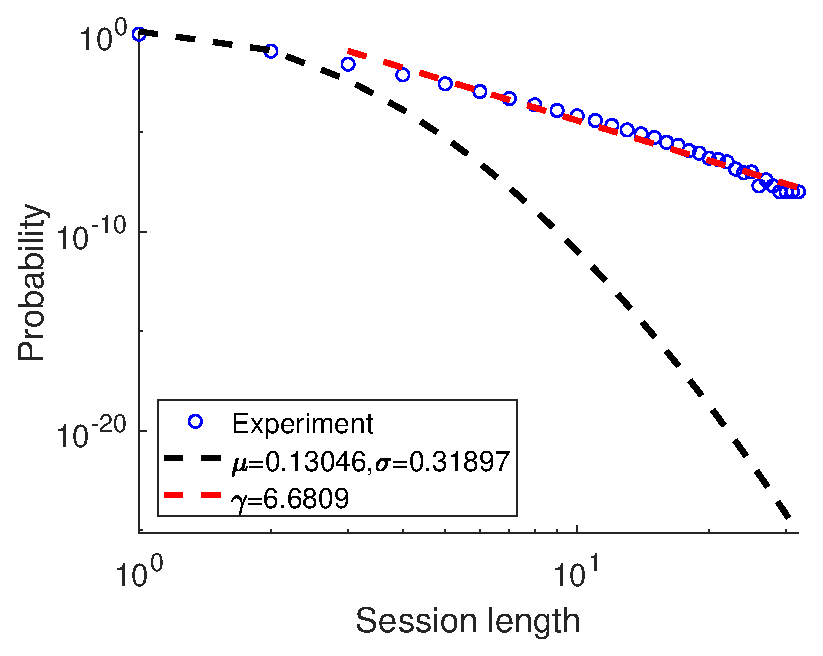
\includegraphics[scale=0.35]{session_count.eps}
\vspace*{-5pt}
\caption{The distribution of session length.}\label{fig:session_len}
\end{figure}

\begin{figure}[htbp]
\centering
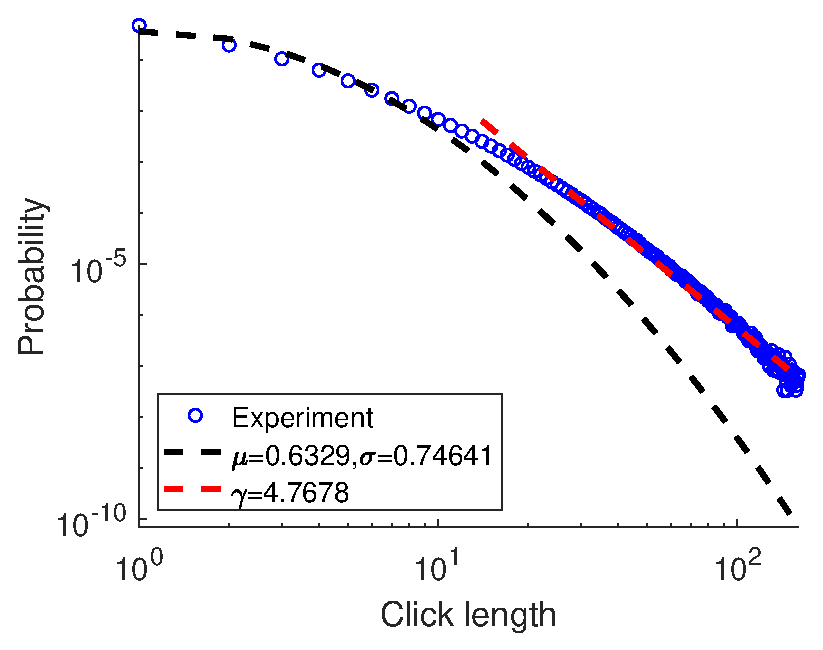
\includegraphics[scale=0.35]{click_count.eps}
\vspace*{-5pt}
\caption{The distribution of click length.}\label{fig:click_len}
\end{figure}

\begin{figure}[htbp]
\centering
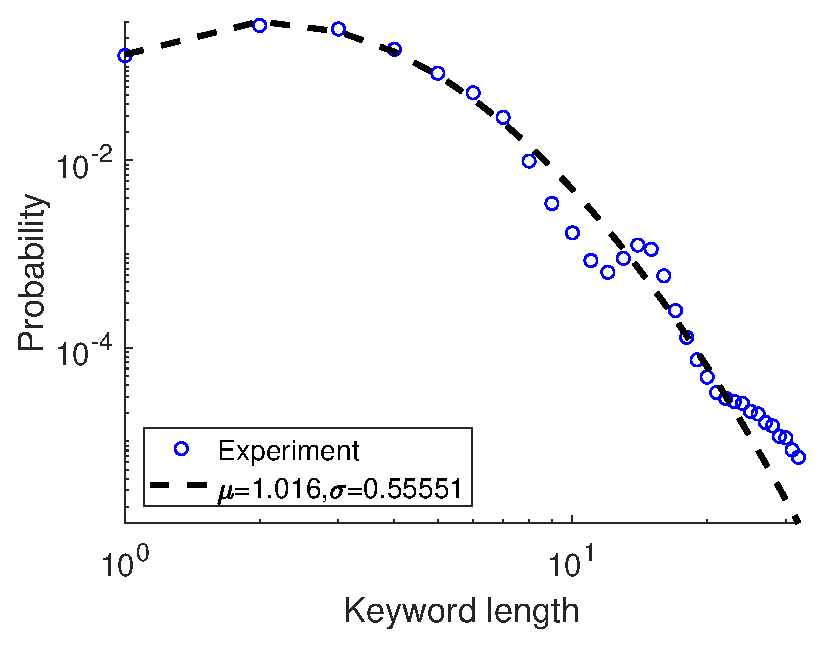
\includegraphics[scale=0.35]{keyword_count.eps}
\vspace*{-5pt}
\caption{The distribution of keyword length.}\label{fig:keyword_len}
\end{figure}

\section{Single Query}\label{sec:single}
Most of the previous work has focused on sessions with multiple queries. But as shown in Tab.~\ref{tab:statistics1}, single query have a very large proportion of all sessions, and we think it is necessary to investigate them separately. In this section, we first combine a variety of features to extract useful search strategies from a single query session. We then connect these strategies and session tags to investigate how different strategies lead to different results.

\subsection{Strategies Extraction}\label{sec:single:strategy}
\begin{table}[htbp]
\centering
\small
\caption{Centroids of the strategy clusters}\label{tab:centroids}
\vspace*{-5pt}
\begin{tabular}{|c|c|c|c|c|c|c|c|c|}
\hline
Cluster & $w_l$ & $c_l$ & $pos$ & $pos_e$ & $seq$ & $seq_e$ & $t$ & $t_e$\\\hline
1 & 2.715 & 1.002 & 1.225 & 0 & 2.118 & 0.001 & 23.303 & 0.001 \\\hline
2 & 4.821 & 1.000 & 1.204 & 0 & 2.212 & 0.001 & 24.501 & 0 \\\hline
3 & 2.891 & 1.007 & 1.865 & 0 & 8.728 & 0.006 & 22.397 & 0 \\\hline
4 & 2.825 & 2.653 & 1.089 & 0 & 4.026 & 0.996 & 26.067 & 0.986 \\\hline
5 & 2.978 & 3.856 & 2.869 & 0.937 & 5.496 & 0.970 & 23.192 & 0.980 \\\hline
6 & 3.561 & 5.172 & 19.693 & 0.813 & 6.204 & 0.805 & 19.051 & 0.830 \\\hline
7 & 3.458 & 12.117 & 5.504 & 0.909 & 5.910 & 0.953 & 19.525 & 0.964 \\\hline
Outlier & 6.584 & 3.274 & 4.121 & 0.945 & 4.724 & 0.934 & 47.384 & 0.946 \\\hline
\end{tabular}
\end{table}

\subsection{Strategies and Tags}\label{sec:single:result}
\begin{table}[htbp]
\centering
\small
\caption{Proportion of tags for each strategy cluster}\label{tab:tags}
\vspace*{-5pt}
\begin{tabular}{|c|c|c|c|}
\hline
Cluster & Add+Purchase & Purchase & Add\\\hline
Average & 0.0739 & 0.0642 & 0.1722 \\\hline 
1 & \textbf{0.0463} & 0.0693 & \textbf{0.1079} \\\hline
2 & \textbf{0.0510} & 0.0755 & \textbf{0.1106} \\\hline
3 & \textbf{0.0343} & \textbf{0.0433} & \textbf{0.0964} \\\hline
4 & \textbf{0.1079} & 0.0841 & 0.1896 \\\hline
5 & \textbf{0.0925} & 0.0507 & \textbf{0.2477} \\\hline
6 & 0.0811 & \textbf{0.0277} & \textbf{0.2640} \\\hline
7 & \textbf{0.1271} & 0.0426 & \textbf{0.4258}\\\hline
Outlier & 0.0950 & 0.0664 & 0.1853\\\hline
\end{tabular}
\end{table}

\section{Multiple Queries}\label{sec:multiple}
\subsection{Motif Finding}\label{sec:multiple:motif}
...
\subsection{Similarity of Query pair}\label{sec:multiple:simila}
...

\section{Predicting search success}\label{sec:predicting}
...

\section{Experiments}\label{sec:experiments}
...

\section{Conclusion}\label{sec:conclusion}
...

\begin{thebibliography}{10}
\bibitem{Silverstein1999Analysis}
C.~Silverstein, H.~Marais, M.~Henzinger and M.~Moricz.
\newblock Analysis of a very large web search engine query log. 
\newblock {\em ACm SIGIR Forum}, 33(1):6-12, 1999.

\bibitem{He2002Combining}
D.~He, A.~G{\"o}ker and DJ.~Harper.
\newblock Combining evidence for automatic web session identification. 
\newblock {\em Information Processing \& Management}, 38(5):727-742, 2002.

\bibitem{Jansen2006How}
BJ.~Jansen, A.~Spink and V.~Kathuria.
\newblock How to define searching sessions on web search engines. 
\newblock In {\em International Workshop on Knowledge Discovery on the Web}, pages 92--109. Springer, 2006.

\bibitem{Jones2008Beyond}
R.~Jones and KL.~Klinkner.
\newblock Beyond the session timeout: automatic hierarchical segmentation of search topics in query logs. 
\newblock In {\em Proceedings of the 17th ACM conference on Information and knowledge management}, pages 699--708. ACM, 2008.

\bibitem{Lucchese2011Identifying}
C.Lucchese, S.~Orlando, R.~Perego, F.~Silvestri and G.~Tolomei.
\newblock Identifying task-based sessions in search engine query logs. 
\newblock In {\em Proceedings of the fourth ACM international conference on Web search and data mining}, pages 277--286. ACM, 2011.

\bibitem{Liao2012Evaluating}
Z.~Liao, S.~Yang, L.~He and Y.~Huang.
\newblock Evaluating the effectiveness of search task trails.
\newblock In {\em Proceedings of the 21st international conference on World Wide Web}, pages 489--498. ACM, 2012.

\bibitem{Cao2009Context}
H.~Cao, DH.~Hu, D.~Shen, D.~Jiang, JT.~Sun, E.~Chen and Q.~Yang.
\newblock Context-Aware Query Classification.
\newblock In {\em Proceedings of the 32nd international ACM SIGIR conference on Research and development in information retrieval}, pages 3--10. ACM, 2009.

\bibitem{Cao2008Context}
H.~Cao, D.~Jiang, J.~Pei, Q.~He, Z.~Liao, E.~Chen and H.~Li.
\newblock Context-Aware Query Suggestion by Mining Click-Through and Session Data.
\newblock In {\em Proceedings of the 14th ACM SIGKDD international conference on Knowledge discovery and data mining}, pages 875--883. ACM, 2008.

\bibitem{Arampatzis2008A}
A.~Arampatzis and J.~Kamps.
\newblock A study of query length.
\newblock In {\em Proceedings of the 31st annual international ACM SIGIR conference on Research and development in information retrieval}, pages 811--812. ACM, 2008.

\bibitem{Kramar2013Personalizing}
T.~Kramar, M.~Barla and M.~Bielikov{\'a}.
\newblock Personalizing Search Using Socially Enhanced Interest Model Built from the Stream of User's Activity. 
\newblock {\em Journal of Web Engineering}, 12(1\&2):65-92, 2013.

\bibitem{Chawla2013kmeans}
S.~Chawla and A.~Gionis.
\newblock $k$-means{-}{-}: A unified approach to clustering and outlier detection.
\newblock In {\em Proceedings of the 2013 SIAM International Conference on Data Mining}, pages 189--197. Society for Industrial and Applied Mathematics, 2013.

\end{thebibliography}
%\balancecolumns
\end{document}
